% Chapter Template

\chapter{Requisits} % Main chapter title

\label{Requisits} % Change X to a consecutive number; for referencing this chapter elsewhere, use \ref{ChapterX}

\section{Propietats i hipòtesis sobre el domini}

Per a poder desenvolupar aquest projecte, s’ha considerat necessari definir una sèrie d’expectatives sobre l’ús del sistema.
\begin{itemize}
\item{}\textbf{Connexió a internet}\\
L’usuari té connexió a internet en tot moment ja que es necessita a l’hora
de guardar i consultar dades, i a l’hora d’accedir a serveis web.
\item{}\textbf{Ús del sistema}\\
Els usuaris utilitzaran el sistema d’acord amb la finalitat per al qual ha
sigut creat sense fer-ne un mal us o emprenen accions malicioses que puguin trencar la integritat del sistema. Tot i així, s’implementaran mitjants de seguretat per protegir l’aplicació en aquest aspecte.
\item{}\textbf{Obtenció de dades correctes}\\
 Les dades que s’obtenen de serveis web són
correctes i actualitzades.

\end{itemize}

\section{Restriccions}
\begin{itemize}
\item[]\textbf{Restricció de la solució}
\begin{itemize}
\item{}Descripció: L’aplicació serà desenvolupada com a aplicació mòbil Android.
\item{}Justificació: Els dispositius mòbils estan sempre aprop de l’usuari i
disponibles per al seu ús, a més, en els últims anys s’ha extés l’ús
d’internet al mòbil. Pel que fa al sistema operatiu, degut a la limitació temporal del treball i a que té una quota de mercat molt gran a
Espanya s’ha optat per la implementació en Android, encara que no
es descarten altres sistemes operatius en un futur.
\end{itemize}
\item[]\textbf{Restricció temporal}
\begin{itemize}
\item{}Descripció: El sistema ha d’estar acabat a meitats de juny de 2017.
\item{}Justificació: S’estableix una data límit per presentar el projecte.
\end{itemize}
\item[]\textbf{Restricció econòmica}
\begin{itemize}
\item{}Descripció: El desenvolupament del projecte es durà a terme sense
cap cost econòmic.
\item{}Justificació: Com que no es disposa de cap inversió econòmica i el
projecte es desenvolupa en un entorn acadèmic les eines i serveis uti-
litzats suposaran un cost molt baix.
\end{itemize}
\end{itemize}

\section{Diagrama de casos d'ús}
En la figura 5.1 es mostra el diagrama de casos d’ús del sistema.

\begin{figure}[!h]
\centering
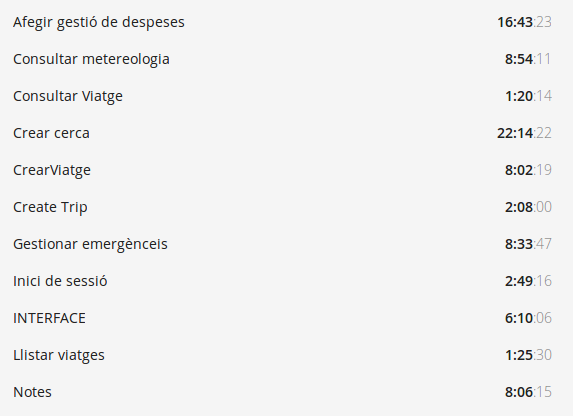
\includegraphics[scale=0.65]{Figures/toggl.jpg}
\caption{Diagrama de casos d'ús}
\end{figure}

\section{Casos dús}

\section{Requisits no funcionals}
